\documentclass[conference]{IEEEtran}
\IEEEoverridecommandlockouts
% The preceding line is only needed to identify funding in the first footnote. If that is unneeded, please comment it out.
\usepackage{cite}
\usepackage{amsmath,amssymb,amsfonts}
\usepackage{algorithmic}
\usepackage{graphicx}
\usepackage{textcomp}
\usepackage{tabularx}
\usepackage{xcolor}
\usepackage{listings}

\lstset{
basicstyle=\small\ttfamily,
columns=flexible,
breaklines=true
}
\def\BibTeX{{\rm B\kern-.05em{\sc i\kern-.025em b}\kern-.08em
    T\kern-.1667em\lower.7ex\hbox{E}\kern-.125emX}}
\begin{document}

\title{Project 24: Suomi24 Mining Health Discussions}

\author{\IEEEauthorblockN{1\textsuperscript{st} Given Name Surname}
    \IEEEauthorblockA{\textit{dept. name of organization (of Aff.)} \\
        \textit{name of organization (of Aff.)}\\
        Oulu, Finland \\
        email address}
    \and
    \IEEEauthorblockN{2\textsuperscript{nd} Given Name Surname}
    \IEEEauthorblockA{\textit{dept. name of organization (of Aff.)} \\
        \textit{name of organization (of Aff.)}\\
        Oulu, Finland \\
        email address}
    \and
    \IEEEauthorblockN{3\textsuperscript{rd} Sercan Turkmen}
    \IEEEauthorblockA{\textit{Center for Machine Vision Research} \\
        \textit{University of Oulu}\\
        Oulu, Finland \\
        sercanturkmen@outlook.com}
    \and
    \IEEEauthorblockN{4\textsuperscript{th} Given Name Surname}
    \IEEEauthorblockA{\textit{dept. name of organization (of Aff.)} \\
        \textit{name of organization (of Aff.)}\\
        Oulu, Finland \\
        email address}
    \and
    \IEEEauthorblockN{5\textsuperscript{th} Given Name Surname}
    \IEEEauthorblockA{\textit{dept. name of organization (of Aff.)} \\
        \textit{name of organization (of Aff.)}\\
        Oulu, Finland \\
        email address}
    \and
    \IEEEauthorblockN{6\textsuperscript{th} Given Name Surname}
    \IEEEauthorblockA{\textit{dept. name of organization (of Aff.)} \\
        \textit{name of organization (of Aff.)}\\
        Oulu, Finland \\
        email address}
}

\maketitle

\begin{abstract}
    This document is a model and instructions for \LaTeX.
    This and the IEEEtran.cls file define the components of your paper [title, text, heads, etc.]. *CRITICAL: Do Not Use Symbols, Special Characters, Footnotes,
    or Math in Paper Title or Abstract.
\end{abstract}

\begin{IEEEkeywords}
    component, formatting, style, styling, insert
\end{IEEEkeywords}

\section{Motivation}
The exploration of medical and health related text has been an important rise a big application for natural language processing and text analysis. It usually helps medical and clinical professionals to identify key parameters and points for decision making. This project aims on exploring such medical related topics in Finland’s popular online forum for free and anonymous discussions, which makes it a good data source for such topics. The anonymity makes users discuss key and vital issues for analysis. The project aims to answer important questions such as identifying main health issues that worries citizens in Finland, their key worries and relieving topics. Identifying how these questions are answered in the text is our challenge that we would like to explore by performing set of tasks that will be explored in details in this paper.

\section{Introduction}
The ability to detect diseases early is paramount to proper treatment. We assume this to be true based on our understanding of the medical field. Therefore finding new ways to detect potential diseases in patients would be extremely beneficial. This project focuses on attempting to create a statistical analysis method to detect potential diseases developing in patients based on their changes in behaviour and communication on online forums. This plan doesn’t limit itself to only one medium, but rather using many channels to try and analyze behaviour, for testing purposes, we focused on Suomi24, largest online social networking website in Finland.

\subsection{Social media analysis and online forums}
During the past years, social media and networking platforms have seen a huge rise in terms of usage between citizens. Social media platforms have been created and developed to easily share material, messages and thoughts with friends and other people around the world. For Finland, The popularity of social network services is also growing: now as many as forty-seven per cent of Finns aged 16 to 74 are registered into various social network services such as Facebook, Twitter, etc. It is also important to mention that according to the same report a third of all Finns follow social network services daily, while of young people and young adults about two thirds visit these services every day. Finns actively share content online and whilst global platforms such as Facebook and YouTube are popular, there are also a number of domestic platforms with many users, such as Suomi24 and IRC-Galleria \cite{finland2015use}. That made Finnish social media a great platform to exchange experiences and knowledge among users online, for example, mobilize supporters in online social media could well be considered an important asset for achieving success in election campaign. The success of an election campaign is to get elected \cite{khaldarova2012publication}. While our focus in this project is to identify key issues related to health in such online platforms.

\subsection{Health mining}
When focusing on social media for health communication, it is useful to first outline the general characteristics of social media. Social media is changing the nature and speed of health care interaction between individuals and health organizations. The general public, patients, and health professionals are using social media to communicate about health issues \cite{thackeray2008enhancing}. Diseases are one of the main issues people share their fight with and ask for help or any other type of support from others. Many health authorities have also started using social media platforms, including, twitter, to communicate directly to patients and interact with them \cite{ventola2014social}. In one review conducted by Stanford, they considered the use and potential of social media and mHealth technologies for cancer prevention, cancer treatment, and survivorship, with clear advantages in broad reach, scaled delivery and low resource setting, health authorities can develop supportive social networks, connect patients and providers, encourage adherence with cancer care, and collect vast quantities of data for advancing cancer research \cite{prochaska2017social}. In this paper, we focus on all health related topics on specific platform in Finnish called Suomi24, which is the most common social online forums in Finland.

\subsection{Natural language processing}
In such sense, the analysis of text is commonly known as natural language processing, which is a subfield of Artificial intelligence that is focused on enabling computers to understand and process human languages, to get computers closer to a human-level understanding of language. Natural language processing has developed through recent years with a great focus on research and industry, through this a lot of tools and products have been released to support text mining and analysis, some trying to build understanding and analysis measures out of text, while other tools used to generate text as well, which is called Natural Language Generation (NLG).

\subsection{Finnish language}
One of our biggest challenges was handling Finnish text and language, for such purpose, we have two approaches, either translate the Finnish text to English and use millions of tools that are easy to tame or use in our application, but translation is not always perfect and sometimes sentences, words or text loses a lot of rich information or translation fails to do the translation due to the existence of unknown characters or undefined text. The other plan is to identify some tools that can handle Finnish text, so we can edit these tools and manage to integrate it in our structure and project.

\section{Tools}
In this section, we discuss the state of art of the tools used in our program and some technical details about it. The main language used in our application is Python and some bash was used as well for tools like FinnPos for lemmatization and morphological tagging. Turku neural dep parser was used for Finnish language besides AFINN for sentiment analysis. Some required features were not supported for Finnish so we had to used some translation APIs like Google translation (googletrans), which were helpful testing some tools as LDA with scikit-learn (countvectorizer) and gensim (construct corpora). A master’s Thesis on Finnish sentiment analysis with Deep Learning helped us to get list of Positive and negative sentiment verbs and adjectives for 81 languages including Finnish. For our Graphical user interface (GUI), we are using Qt5 to make an application to run the functions.

\subsection{NLTK}
Famous tool is Python based Natural Language Processing Toolkit (NLTK) which provides a lot of applications and solutions to text analysis like sentiment analysis, categorization, classification, information extraction, tokenizing, part of speech tagging, parsing and many others. NLTK is written in Python and distributed under the GPL open source license. a broad-coverage natural language toolkit that provides a simple, extensible, uniform framework for assignments, demonstrations and projects. It is thoroughly documented, easy to learn, and simple to use. Over the past three years, NLTK has become popular in teaching and research \cite{bird2004nltk}.

\subsection{Gensim}
Gensim also is a free open source code for text analysis, it’s main target is to model topics out of free text, it follows an unsupervised semantic modeling from plain text. Latent Dirichlet allocation (LDA) is used to extract topics from texts using predetermined training material \cite{qiu2014topic}. It is a matter of questioning how we are going to use this model to extract topics and what will affect on our process after extracting topics, taking in consideration that text is in Finnish. So, we had two approaches, either translate the text into English and then perform the LDA topic modeling or use it directly on Finnish text. The complications here were the size of the dataset which played a huge role affecting the translation process due to the limitations stated by the Google API \cite{aiken2011analysis}.

\subsection{Polyglot}
One of the many challenges to face when dealing with non English text is checking for support for these languages such as Finnish. Polyglot provides support to many languages depending on the feature required \cite{al2013polyglot}. We used Polyglot on Finnish text to get named entities, which can detect locations, organization and persons entities and supports 40 major languages \cite{al2015polyglot}.

\subsection{Stanford tools}
Stanford university have been developing many tools in the field of natural language processing. It is an extensible annotation-based NLP pipeline that provides core natural language analysis. This toolkit is quite widely used, both in the research NLP community and also among commercial and government users of open source NLP technology. It provides named entity detection and part of speech tagging as two of the important features provided by Stanford tools which are used extensively \cite{manning2014stanford}.

\subsection{Turku parsers}
A neural parsing pipeline for segmentation, morphological tagging, dependency parsing and lemmatization with pre-trained models for more than 50 languages, using Parser v2 and universal-lemmatizer (which uses Neural model for lemmatization using OpenNMT and pytorch libraries). Turku dep parser take over, the new pipeline is fully neural, it provides better accuracy, fast when parsing large documents, with about 5x faster than the previous Finnish-dep-parser as it takes advantage of GPU, the only downside for it is the long start-up cost when it’s loading the models \cite{kanerva2018turku}.

\begin{figure}[htbp]
    \centerline{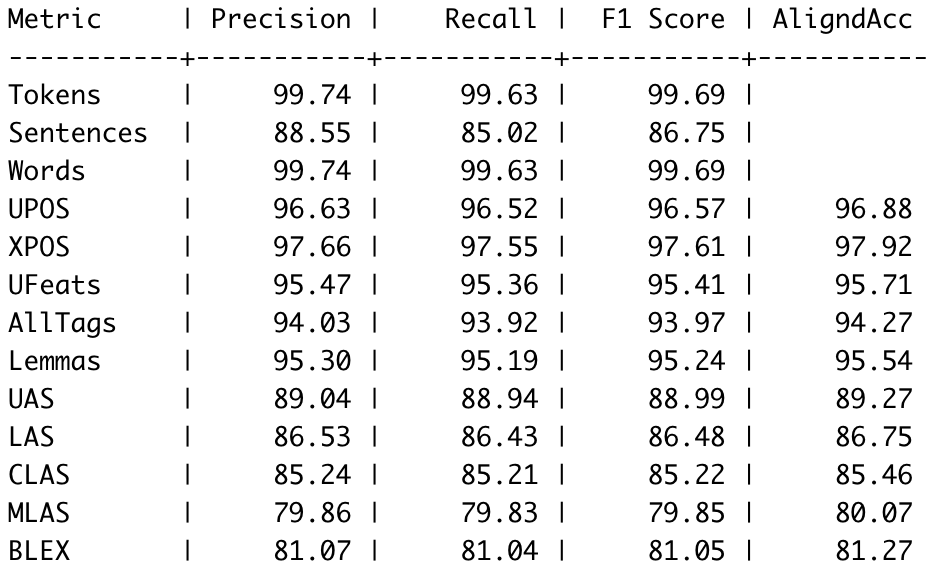
\includegraphics[width=0.45\textwidth]{figures/fig1.png}}
    \caption{Turku parser performance metrics.}
    \label{turku_parser_performance}
\end{figure}

\begin{figure}[htbp]
    \centerline{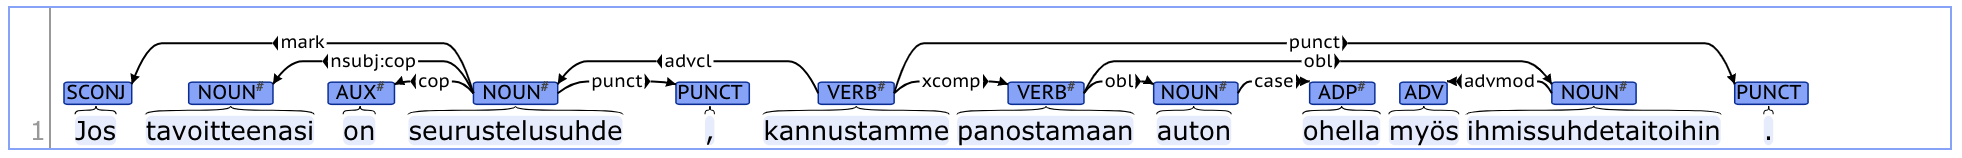
\includegraphics[width=0.45\textwidth]{figures/fig2.png}}
    \caption{Example visual from the output of turku parser.}
    \label{turku_parser_example}
\end{figure}

\subsection{Afinn}
Sentiment analysis tools are abundant for English text, but not much for other languages as Finnish, one of the simplest sentiment analysis approaches compares the words of a posting against a labeled word list, where each word has been scored for valence, a “sentiment lexicon” or “affective word lists” [13]. This tool provides a manually labelled list of words which are then used in evaluating free-text sentiment by matching the text to the list. We were able to construct our own list in Finnish, making the tool available to be used for Finnish text.

\section{Implementation}

\subsection{Tasks}
\begin{itemize}
    \item Extract health related topics from Suomi24
    \item Analyze frequency of named entities and categorize them based on a taxonomy
    \item Use parser tree on sentences with 30 most repeated named entities found
    \item Analyze frequencies of co-occurring pairs of words in threads and comments
    \item Use sentiment analyzer for global sentiment
    \item Compile set of verbs / adjectives with negative / positive sentiment
    \item Classify threads per year and get year variation
    \item LDA topic detection
    \item Identify diseases and get top ones
    \item More analysis on every disease
    \item GUI
\end{itemize}

\subsection{Task 1: Dataset}
To analyze suomi24, we looked for options to get the dataset from the website, either scraping the online forum or look for their dataset online, we were able to use the online corpus provided by university of Helsinki, which had all discussions from 2001 till June 2015 with around 231 million sentences. As our focus is health related topics online, we looked for ‘Terveys’ subtopic which means health in Finnish, compared to other approach which is catching topics from the forum using word matching with a list of health related keywords, subtopic extraction enabled us to get a relatively big dataset of specifically health discussions with less noise in the dataset. The final dataset was around 28 thousand sentences to be used for actual analysis. To make it easier for our future tasks, we developed an architecture to help us progress in such project. The architecture discussed in Figure 1, explains how codes and tools will be used in the next steps to achieve the target. Such architecture will be helpful for future modifications and will provide a good structure for our codes.

\subsubsection{Pre-processing of Suomi24 data}
The data in Suomi24 text dumps was supplied in JSON format and the storage size of the raw data was about 15 gigabytes. The structure of the data is shown in figures \ref{message_data_example}, \ref{message_data_structure}, \ref{comment_data_structure}, \ref{topic_data_structure}.

\begin{figure}[htbp]
    \begin{lstlisting}
{
    "body":"<p>Niin k\u00e4ynki ens
            kerralla! Niin kannattaa
            teh\u00e4 muittenki. Tai
            hakea K\u00e4rkk\u00e4iselt
            \u00e4.</p>",
    "quote_id":65033569,
    "deleted":false,
    "created_at":1388253658000,
    "comment_id":65288763,
    "anonnick":"kuparia kuparia",
    "thread_id":11858119,
    "parent_comment_id":65032642
}
\end{lstlisting}
    \caption{Suomi24 message data example.}
    \label{message_data_example}
\end{figure}

\begin{figure}[htbp]
    \begin{lstlisting}
{
    "body": STRING,
    "title": STRING,
    "deleted": BOOLEAN,
    "views": INT,
    "anonnick": STRING,
    "thread_id": INT,
    "closed": BOOLEAN,
    "created_at": INT,
    "Topics": [
        {TOPIC_1},
        ...
        {TOPIC_N}
    ],
    "comments": [
        (array of COMMENT format)
    ]
}
\end{lstlisting}
    \caption{Suomi24 message data structure example.}
    \label{message_data_structure}
\end{figure}

\begin{figure}[htbp]
    \begin{lstlisting}
{
    {MESSAGE}
    "quote_id": INT,
    "comment_id": INT,
    "parent_comment_id": INT
}
\end{lstlisting}
    \caption{Suomi24 comment data structure example.}
    \label{comment_data_structure}
\end{figure}

\begin{figure}[htbp]
    \begin{lstlisting}
{
  "title": STRING,
  "topic_id": INT
}
\end{lstlisting}
    \caption{Suomi24 topic data structure example.}
    \label{topic_data_structure}
\end{figure}

\begin{figure}[htbp]
    \centerline{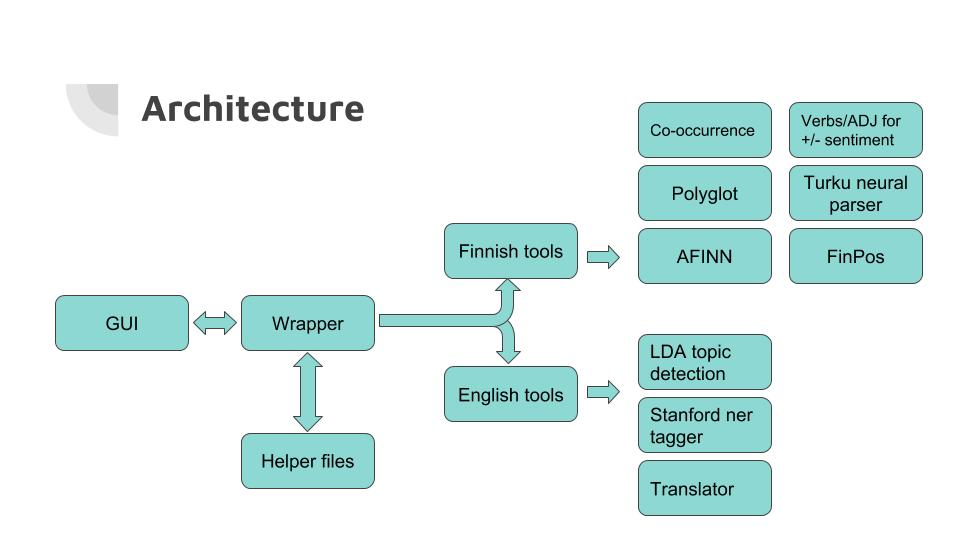
\includegraphics[width=0.45\textwidth]{figures/fig3.jpg}}
    \caption{Implementation architecture.}
    \label{implementation_architecture}
\end{figure}

The body text included some HTML tags for formatting, for example:

\textless p\textgreater ai huh että se arvon on oltava nykyään 21e!! No jo nyt on, mutta hyvä kuulla että tämä ei nyt ylitsepääsemättömän vaikeaa pitäisi olla ja tiedänpähän toiste että en varmaan sitten kyllä mitään ulkomailta tilaa ainakaan siis eun ulkopuolelta\textless /p\textgreater

\subsubsection{Preprocessing of Finnish text}
After careful analysis the it was concluded that the best format to conduct the tasks was a month divided, lemmatized text format. So, the following steps were made for pre-processing:

\begin{itemize}
    \item Filtering of data threads only to take “Terveys” (eg. “Health”) topics into account.
    \item Conversion of JSON message body data into new line divided raw text files. File names: month-year.txt. All metadata was stripped.
    \item Removal of HTML tags from body text
    \item Conversion of text to have each word on a new line.
    \item Using the FinnPos ftb-label tagger, lemmatized the newline separated texts
    \item Using cut and sed tools on Linux bash, stitched the lemmatized, newline separated words back to sentences.
\end{itemize}

Example of lemmatization for one sentence:

\textit{\textbf{Original:} itse tyrkytän asiantuntijan kautta lääkevalmisteita tai valittuja käsikaupan tuotteita , kuten vitamiinilisät. moni tyrkyttää kemikaalien yhdistelmiä esim mäkikuismaaetc ... kiitos haastavasta tehtävästä.}

\textit{\textbf{Lemmatized:}itse tyrkyttää asiantuntija kautta lääkevalmiste tai valita käsikauppa tuote , kuten vitamiinilisät moni tyrkyttää kemikaali yhdistelmä esim mäkikuismaaetc ... kiitos haastaa tehtävä.}

A quick analysis on this one sentence shows that there are spelling mistakes in the original (“mäkikuismaaetc”) and the lemmatization was not performed on all words (“vitamiinilisät” should ne lemmatized to “vitamiinilisä”). Despite this, overall the FinnPos tagger did a great job.

\subsection{Task 2: Named entities analysis}
Next task was to analyze the frequency of named entities in the resulted threads, first to analyze the overall repetition of named entities in the whole dataset. As shown in figure 2, location (LOC), person (PER) and organization (ORG) are the entities detected, while the figure represents thirty most repeated ones, obviously here locations make most of the named entities detected.

\begin{figure}[htbp]
    \centerline{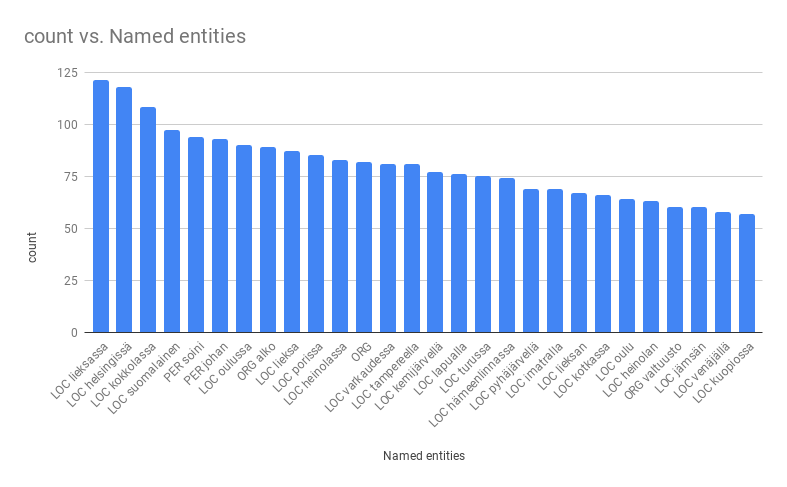
\includegraphics[width=0.45\textwidth]{figures/fig4.png}}
    \caption{Frequency of 30 highest named entities.}
    \label{frequency_of_30_highest_named_entities}
\end{figure}

\subsection{Task 3: Parser tree}
Figures from \ref{parser_tree_on_30_most_common_named_entities} shows samples from sentences that contains one of these most repeated named entities. Using Turku neural parser, we were able to visualize these sentences and identify common verbs and adjectives associated with them.

\begin{figure}[htbp]
    \centerline{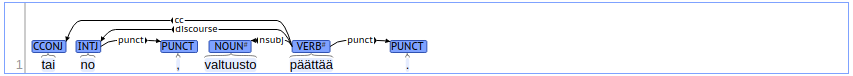
\includegraphics[width=0.45\textwidth]{figures/fig5.png}}
    \centerline{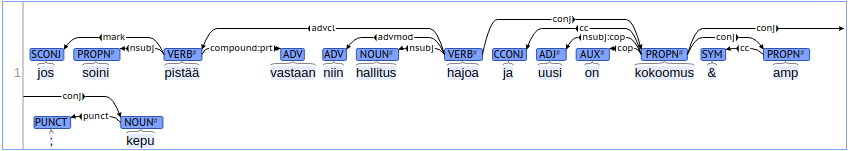
\includegraphics[width=0.45\textwidth]{figures/fig7.png}}
    \centerline{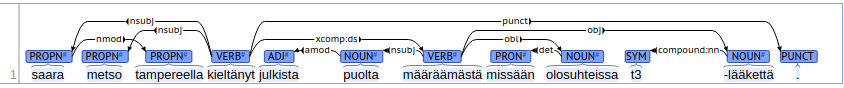
\includegraphics[width=0.45\textwidth]{figures/fig8.png}}
    \centerline{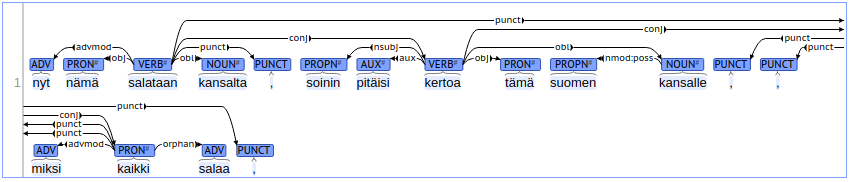
\includegraphics[width=0.45\textwidth]{figures/fig9.png}}
    \caption{Parser tree on 30 most common named entities.}
    \label{parser_tree_on_30_most_common_named_entities}
\end{figure}
\clearpage

\subsection{Task 4: Most repeated co-occurrences}

\begin{figure}[hbtp]
    \centerline{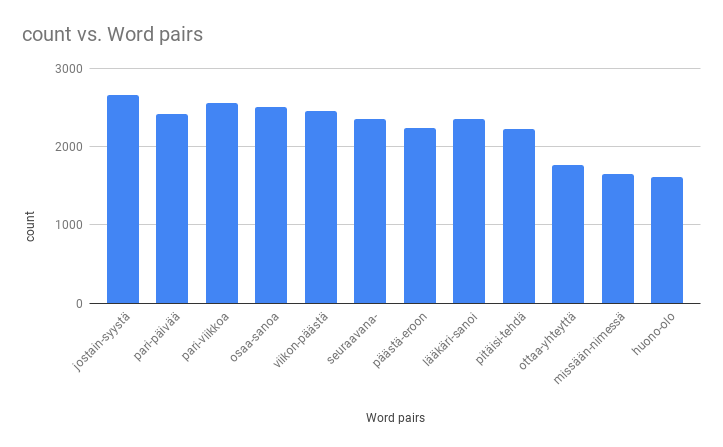
\includegraphics[width=0.45\textwidth]{figures/fig12.png}}
    \caption{Count vs. word pairs.}
    \label{count_vs_word_pairs}
\end{figure}

\subsection{Task 5: Overall sentiment analysis}

\begin{figure}[htbp]
    \centerline{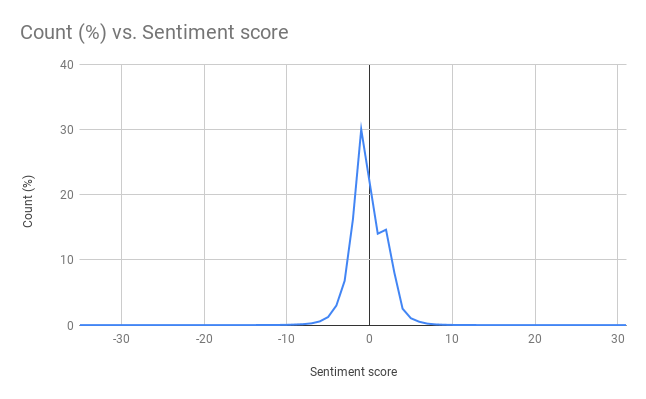
\includegraphics[width=0.45\textwidth]{figures/fig13.png}}
    \caption{Count (\%) vs. Sentiment score.}
    \label{count_percent_vs_sentiment_score}
\end{figure}

\subsection{Task 8: Sentiment analysis over time}

\begin{figure}[htbp]
    \centerline{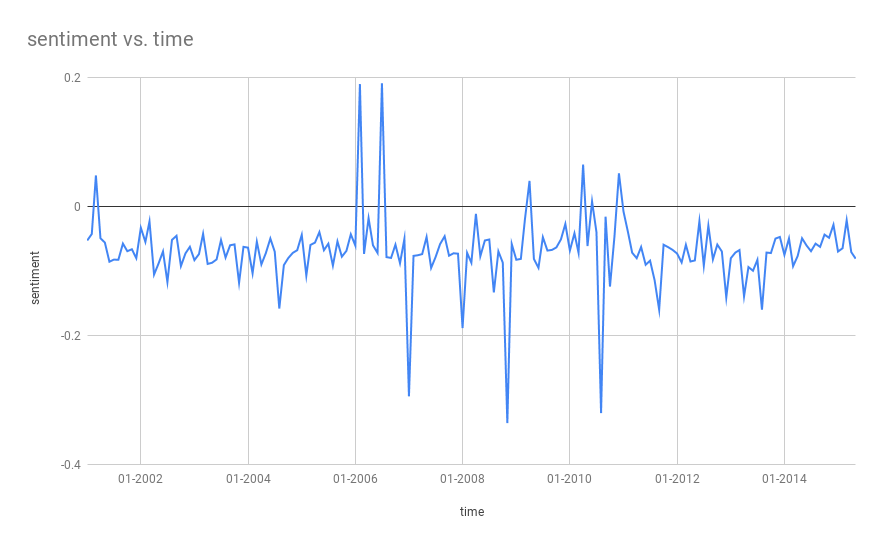
\includegraphics[width=0.45\textwidth]{figures/fig14.png}}
    \caption{Sentiment analysis over time.}
    \label{sentiment_analysis_over_time}
\end{figure}

\clearpage

\subsection{Task  9: Comparison of LDA topic detection results for three month data with and without lemmatization of source data}

\begin{table}[htbp]
    \caption{Without lemmatization}
    \begin{center}
        \begin{tabularx}{\linewidth}{| l | X |}
            \hline
            Year & Topics \\
            \hline
            11-2003 & päättyi, päässä, päässäni, päätöksiä, päättäjien, päättäjiä, päättäjähän, päättäjät, päättäneet, päättäny, päättävät, päättää, päätynyt, päätyy, päätä, päätäsi, päätökset, päätteeksi, päässäsi, päästä, ja, ei, että, mutta, kun, niin, se, ole, quot, jos, en, olen, voi, myös, oli, kuin, tai, mitä, olla \\
            \hline
            12-2014 & päätettiin, päätettävissään, päätelmänne, päätetiin, päätethään, päätethin, pääterveyskeskus, pääterveysasemalla, pääterveysasemaa, päätepysäkki, päätepisteeseensä, päätepiste, päätema, pääteltävissä, päätelmään, päätelmää, päätelmät, päätettävä, päätettävissä, ja, ei, että, se, kun, quot, niin, ole, jos, mutta, oli, tai, nyt, kuin, en, voi, sen, olla \\
            \hline
            04-2009 & pääomareservit, pääsevät, pääomistajahan, pääosin, pääpuoleen, pääpuoskarit, päärynä, pääse, pääsee, pääseekö, pääseeköhän, pääseminen, pääsemästä, pääsemättömältä, pääsemään, pääsen, pääset, pääomaköyhintä, pääneuvottelija, päänsä, ja, ei, että, se, mutta, kun, niin, quot, ole, jos, olen, en, oli, nyt, tai, sitten, myös, voi, sen\\
            \hline
        \end{tabularx}
        \label{without_lemmatization}
    \end{center}
\end{table}

\begin{table}[htbp]
    \caption{With lemmatization}
    \begin{center}
        \begin{tabularx}{\linewidth}{| l | X |}
            \hline
            Year & Topics \\
            \hline
            12-2014 & pyydyksiä, pyyhkiminen, pyydys, pysäyttää, pyydetään, pyydetty, pyydellä, pyyde, pyy, pytä, pytytyä, pytyn, pyttyy, pyttymäinen, pytty, pyttis, pyttipannu, pyydystäjä, pyyhkimään, pyyhkii, quo, voida, tehdä, mennä, ihminen, käydä, ottaa, tietää, haluta, sanoa, kaupunki, työ, päivä, mies, raha, suomi, maksaa, kunta\\
            \hline
            04-2009 & pysäköintialue, pysähtyä, pysähtytyä, pysähtyneisyys, pysähtyneen, pysähdys, pysyä, pysyvät, pysyvästi, pysyvä, pysytellä, pysyntyä, pysyikö, pysyi, pysy, pystyä, pystyyn, pysäköintihalli, pysäkki, pysäköinti, voida, quo, mennä, tehdä, tietää, käydä, ihminen, käyttää, päivä, ottaa, lääkäri, sanoa, haluta, tuntua, aiheuttaa, syödä, päästä, lääke, elämä\\
            \hline
        \end{tabularx}
        \label{with_lemmatization}
    \end{center}
\end{table}

\begin{table}[htbp]
    \caption{Topic detection without lemmatization}
    \begin{center}
        \begin{tabularx}{\linewidth}{| l | X |}
            \hline
            Year & Topics \\
            \hline
            11-2003 & päättyi, päässä, päässäni, päätöksiä, päättäjien, päättäjiä, päättäjähän, päättäjät, päättäneet, päättäny, päättävät, päättää, päätynyt, päätyy, päätä, päätäsi, päätökset, päätteeksi, päässäsi, päästä, ja, ei, että, mutta, kun, niin, se, ole, quot, jos, en, olen, voi, myös, oli, kuin, tai, mitä, olla\\
            \hline
            12-2014 & päätettiin, päätettävissään, päätelmänne, päätetiin, päätethään, päätethin, pääterveyskeskus, pääterveysasemalla, pääterveysasemaa, päätepysäkki, päätepisteeseensä, päätepiste, päätema, pääteltävissä, päätelmään, päätelmää, päätelmät, päätettävä, päätettävissä, ja, ei, että, se, kun, quot, niin, ole, jos, mutta, oli, tai, nyt, kuin, en, voi, sen, olla\\
            \hline
            04-2009 & pääomareservit, pääsevät, pääomistajahan, pääosin, pääpuoleen, pääpuoskarit, päärynä, pääse, pääsee, pääseekö, pääseeköhän, pääseminen, pääsemästä, pääsemättömältä, pääsemään, pääsen, pääset, pääomaköyhintä, pääneuvottelija, päänsä, ja, ei, että, se, mutta, kun, niin, quot, ole, jos, olen, en, oli, nyt, tai, sitten, myös, voi, sen\\
            \hline
        \end{tabularx}
        \label{topic_detection_without_lemmatization}
    \end{center}
\end{table}

\begin{table}[htbp]
    \caption{Topic detection with lemmatization}
    \begin{center}
        \begin{tabularx}{\linewidth}{| l | X |}
            \hline
            Year & Topics \\
            \hline
            12-2014 & pyydyksiä, pyyhkiminen, pyydys, pysäyttää, pyydetään, pyydetty, pyydellä, pyyde, pyy, pytä, pytytyä, pytyn, pyttyy, pyttymäinen, pytty, pyttis, pyttipannu, pyydystäjä, pyyhkimään, pyyhkii, quo, voida, tehdä, mennä, ihminen, käydä, ottaa, tietää, haluta, sanoa, kaupunki, työ, päivä, mies, raha, suomi, maksaa, kunta\\
            \hline
            11-2013 & pystyis, pyssymestari, pyssy, pyssätä, pyssyä, pystynyt, pystyisi, pystyisikä, pystyisikään, pystyisit, ei, pystyitää, pystykahvi, pystykkä, pystykuolema, pystykä, pystymätön, pystyneet, pystyidä, pyssystään, jooh, pyssyyn, suanoo, quo, voida, tehdä, mennä, ihminen, käydä, ottaa, tietää, sanoa, haluta, päivä, työ, mies, päästä, maksaa, raha, kaupunki, käyttää, paikka\\
            \hline
            04-2009 & pysäköintialue, pysähtyä, pysähtytyä, pysähtyneisyys, pysähtyneen, pysähdys, pysyä, pysyvät, pysyvästi, pysyvä, pysytellä, pysyntyä, pysyikö, pysyi, pysy, pystyä, pystyyn, pysäköintihalli, pysäkki, pysäköinti, voida, quo, mennä, tehdä, tietää, käydä, ihminen, käyttää, päivä, ottaa, lääkäri, sanoa, haluta, tuntua, aiheuttaa, syödä, päästä, lääke, elämä\\
            \hline
        \end{tabularx}
        \label{topic_detection_with_lemmatization}
    \end{center}
\end{table}

\begin{figure}[htbp]
    \centerline{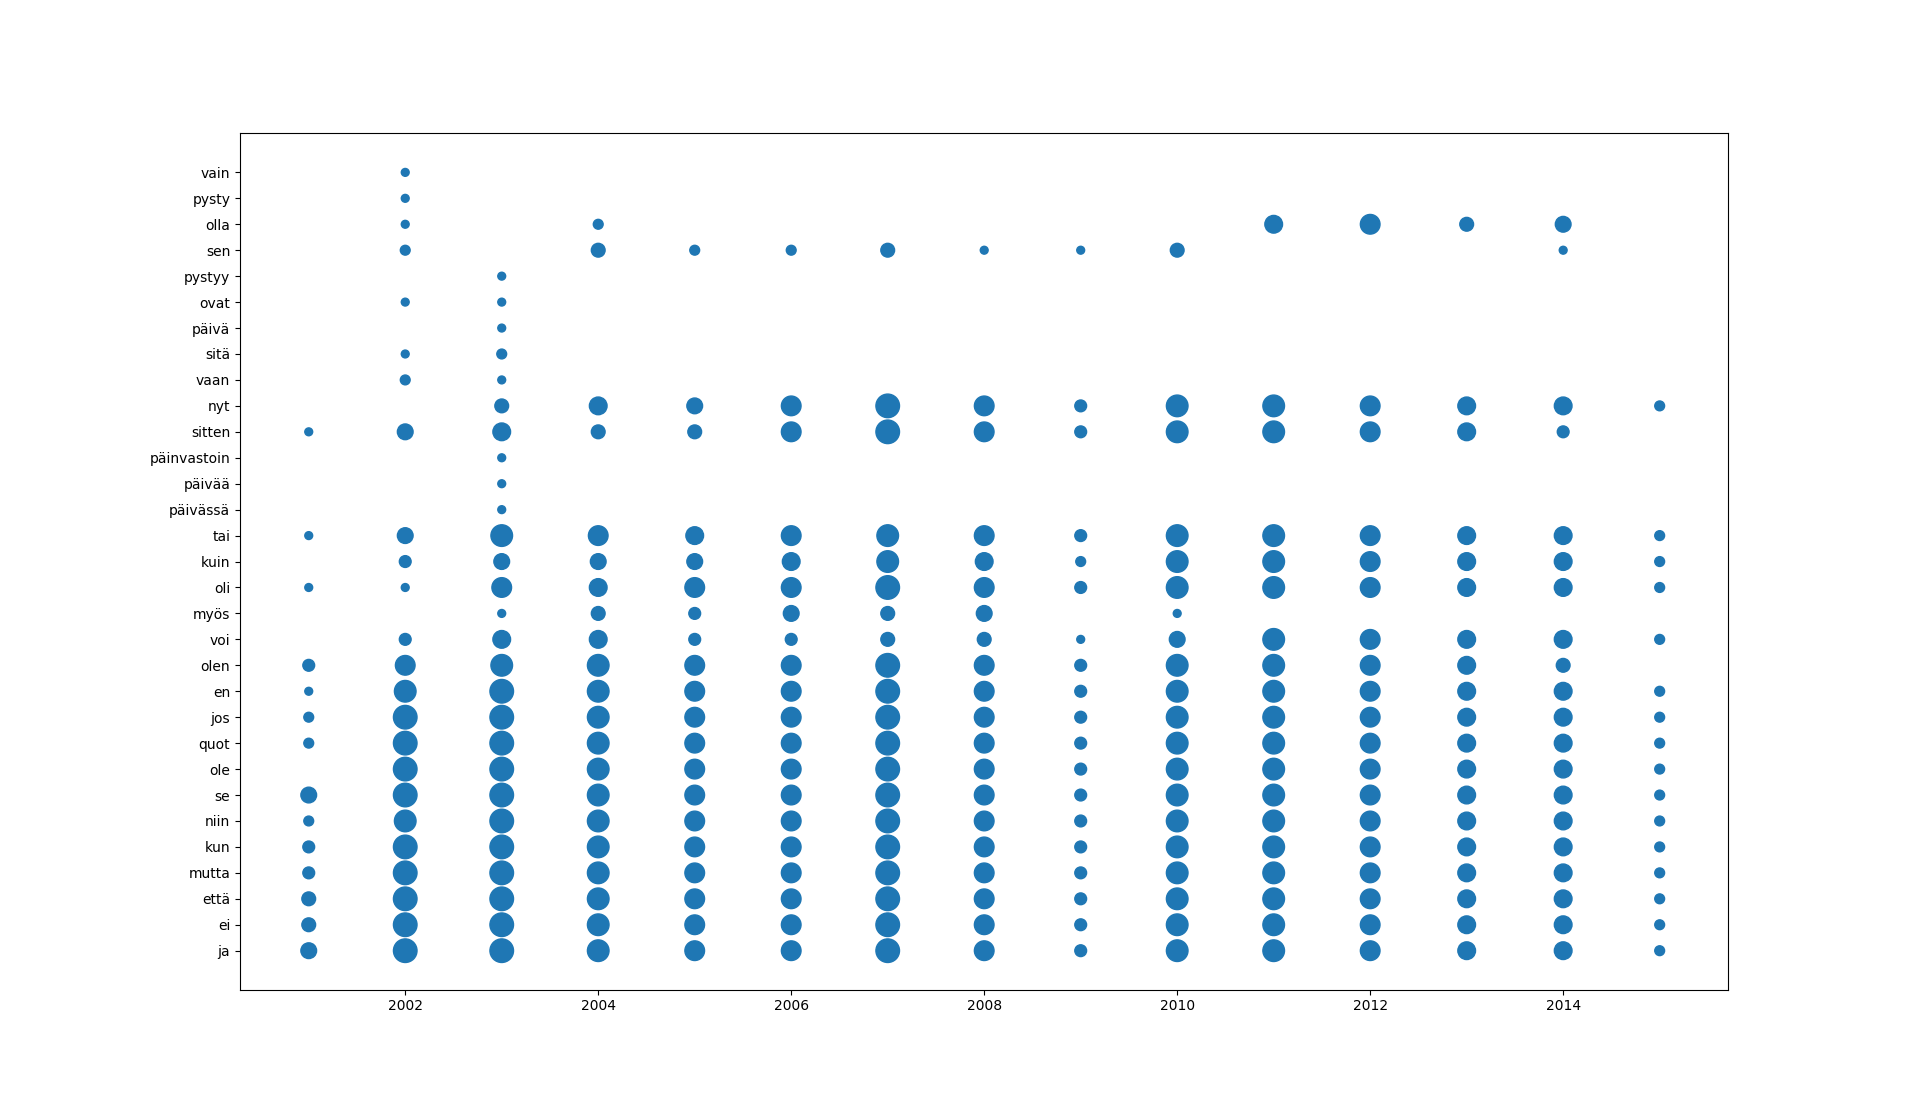
\includegraphics[width=0.5\textwidth]{figures/fig15.png}}
    \caption{Without lemmatization topics.}
    \label{without_lemmatization_topics}
\end{figure}

\begin{figure}[htbp]
    \centerline{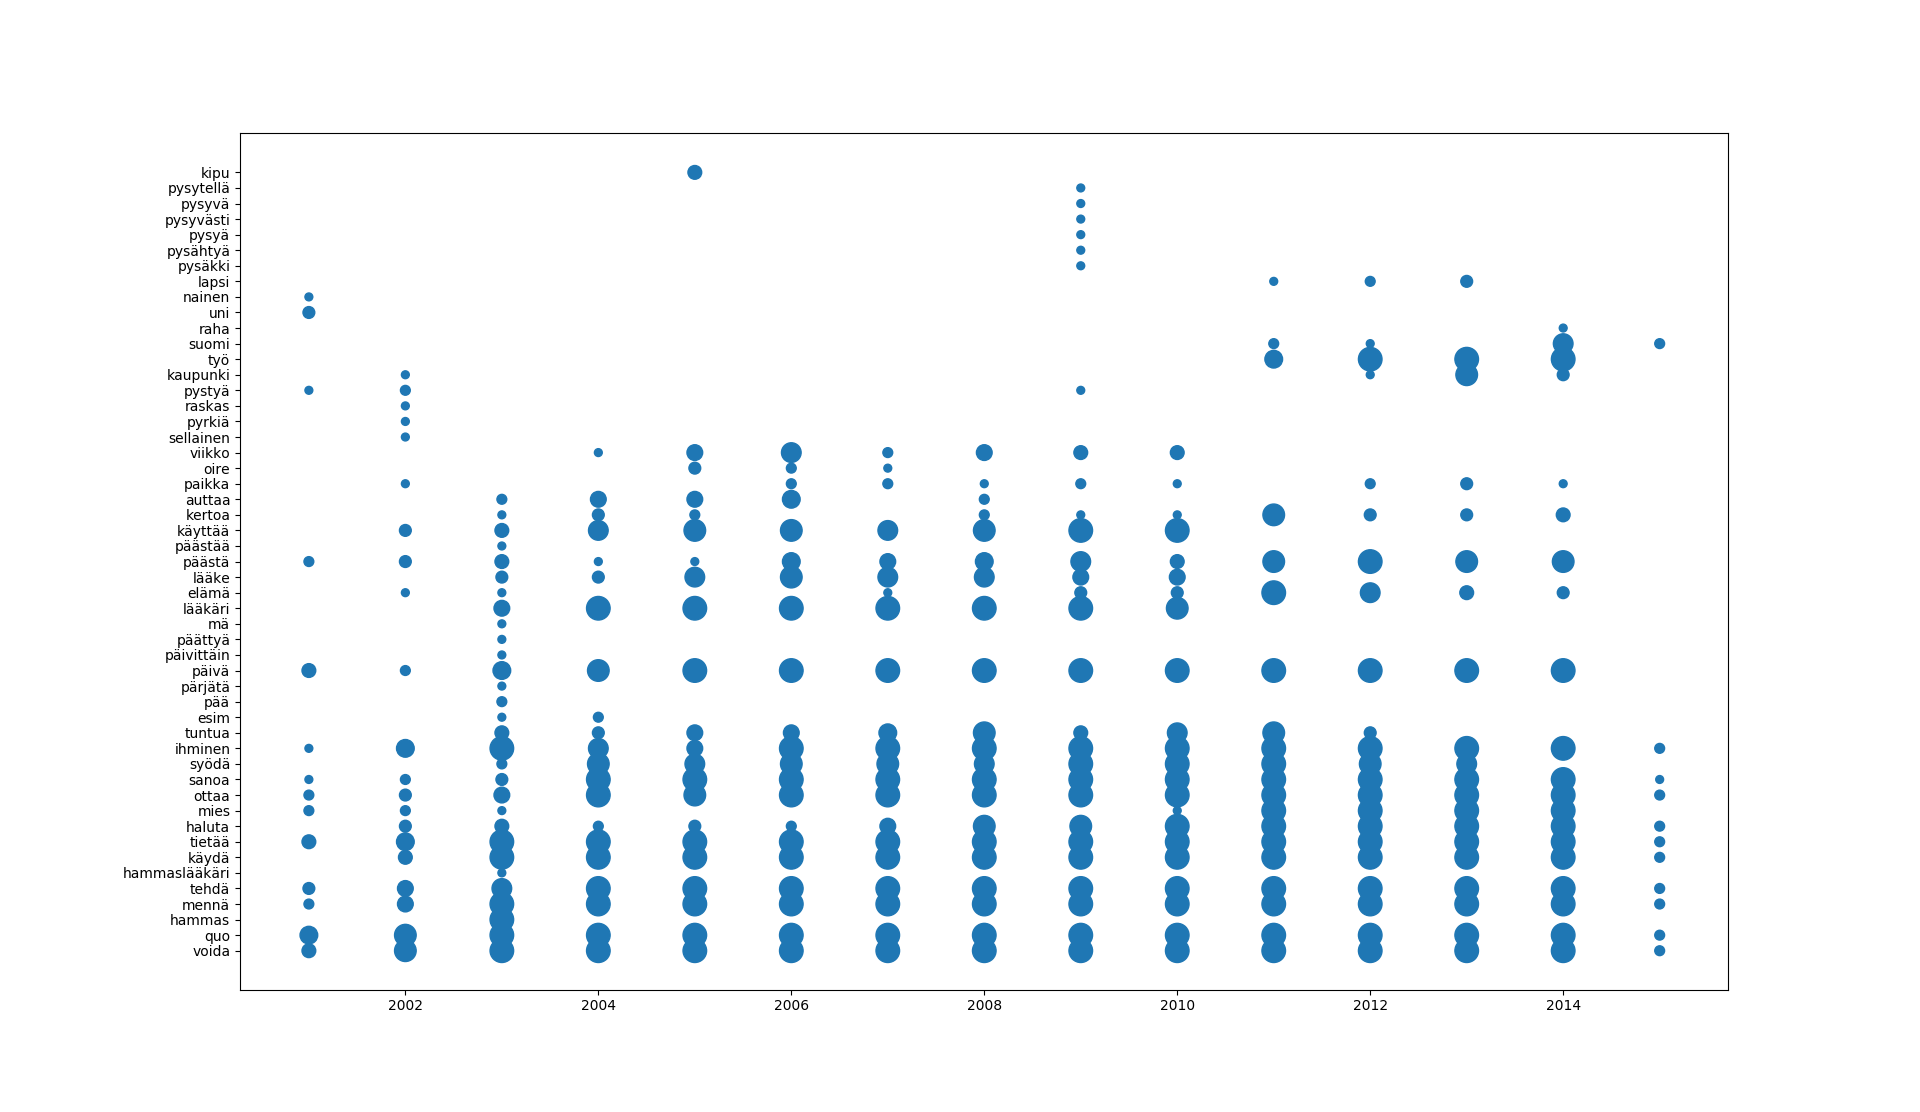
\includegraphics[width=0.5\textwidth]{figures/fig16.png}}
    \caption{With lemmatization topics.}
    \label{with_lemmatization_topics}
\end{figure}







\subsection{Task 10 and 11: Progress on disease detection from ontology}

Quick and dirty way to get Finnish health related words (49131 in total) from TERO Terveyden ja Hyvinvoinnin Ontologia:
\begin{lstlisting}
# wget https://finto.fi/rest/v1/tero/data?format=application/rdf%2Bxml
# cat tero-skos.rdf | grep lang=\"fi\" | sed 's/<[^>]\+>//g' | tr -d ' ' | sed '/^YSO/ d' > finnish-words-in-file.txt
\end{lstlisting}

Polyglot Finnish Part-of-Speech detection and categorization of Finnish sentiment words (positive and negative):
\begin{lstlisting}
# polyglot --lang fi tokenize --input finnish_toolkit/negative_words_fi.txt |  polyglot --lang fi pos | grep VERB | tr -d ' ' | tr -d 'VERB' > negative_verbs.txt
\end{lstlisting}

Conversion of a 100MB Suomi24 JSON file to a file with each word separated on a newline without tags and punctuation:
\begin{lstlisting}
# cat dump05500-05599.json | jq . | jq .[].body | tr -d '<p>' | tr -d '</p>' | sed 's/^.\(.*\).$/\1/' | tr -d '[:punct:]'| xargs -n1 > one-word-per-line-no-punctuation.txt
\end{lstlisting}

Lemmatization of the data from previous step with FinnPOS (ftb-label):
\begin{lstlisting}
# cat one-word-per-line-no-punctuation.txt | ftb-label > lemmatized.txt
# cut -f3 lemmatized.txt > output.txt
\end{lstlisting}

Output is a lemmatized, new line separated word list from the original data.

In tasks 10 and 11, it stated “Identify the various diseases mentioned in the dataset both as separate threads or mentioned in the core document and Repeat the time analysis by reporting the main frequency of diseases discussed per month / year”.

The following steps were taken to solve this task:
\begin{itemize}
    \item Generate disease vocabulary in Finnish
    \item Match disease vocabulary to lemmatized Suomi24 data per month
    \item Generate year and total occurrences
    \item Normalize the number of monthly and yearly occurrences of diseases with the amount of messages for each month and year
\end{itemize}

All operations where performed on the Linux command line with sed, cut, etc. tools. Disease vocabulary was obtained from the FinnMesh Medical Subject Headings ontology. The ontology also includes a lot of other health related words. Overall the vocabulary was 80k words and it was generated matching “prefLabel” and “altLabel” tags of the mesh-skos.rdf file.

Matching this amount of words to monthly Suomi24 data proved to be too time consuming, so filtering of the vocabulary was needed.

Disease vocabulary filtering process:
\begin{itemize}
    \item Match the 80k word disease vocabulary to one month of Suomi24 data. This step took about 20 minutes.
    \item Count the number of occurrences per word.
    \item Remove words which have 0-2 occurrences.
\end{itemize}

As a result the vocabulary was reduces from 80k to a much more manageable 1722 words. Even in this list the number of words directly related to diseases was small.

\section{Results}

\begin{figure}[htbp]
    \centerline{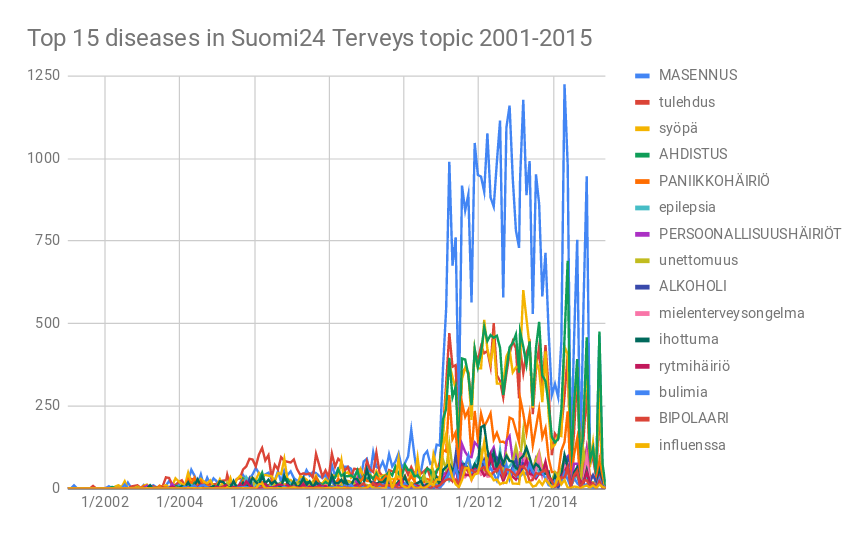
\includegraphics[width=0.45\textwidth]{figures/fig17.png}}
    \caption{Top 15 diseases in Suomi24 Terveys topic 2001-2015.}
    \label{top_15_diseases_in_suomi24_terveys_topic_2001_2015}
\end{figure}

\begin{figure}[htbp]
    \centerline{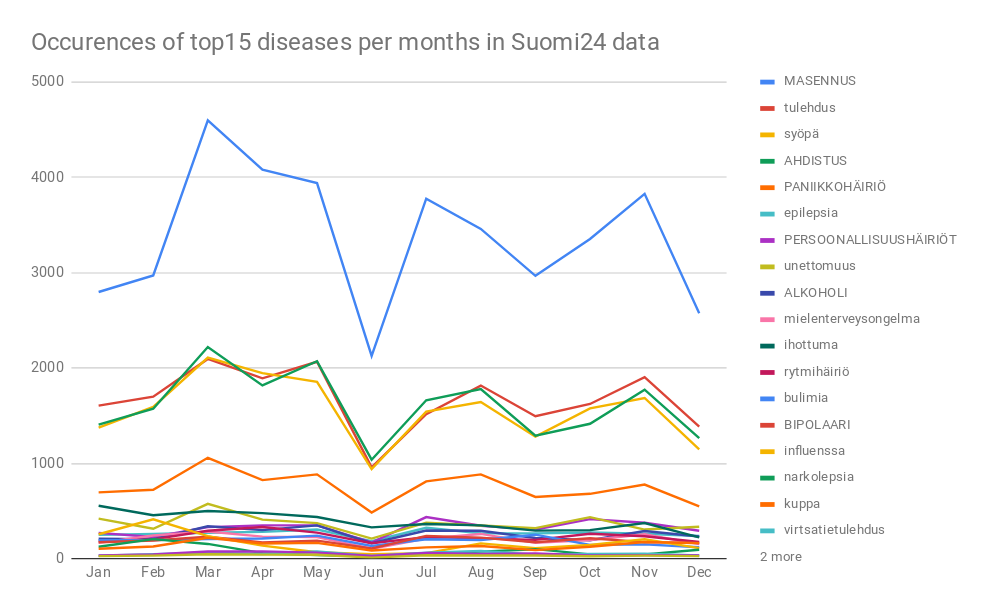
\includegraphics[width=0.45\textwidth]{figures/fig18.png}}
    \caption{Occurences of top15 diseases per month in Suomi24 data.}
    \label{occurences_of_top15_diseases_per_month_in_suomi24_data}
\end{figure}

\begin{figure}[htbp]
    \centerline{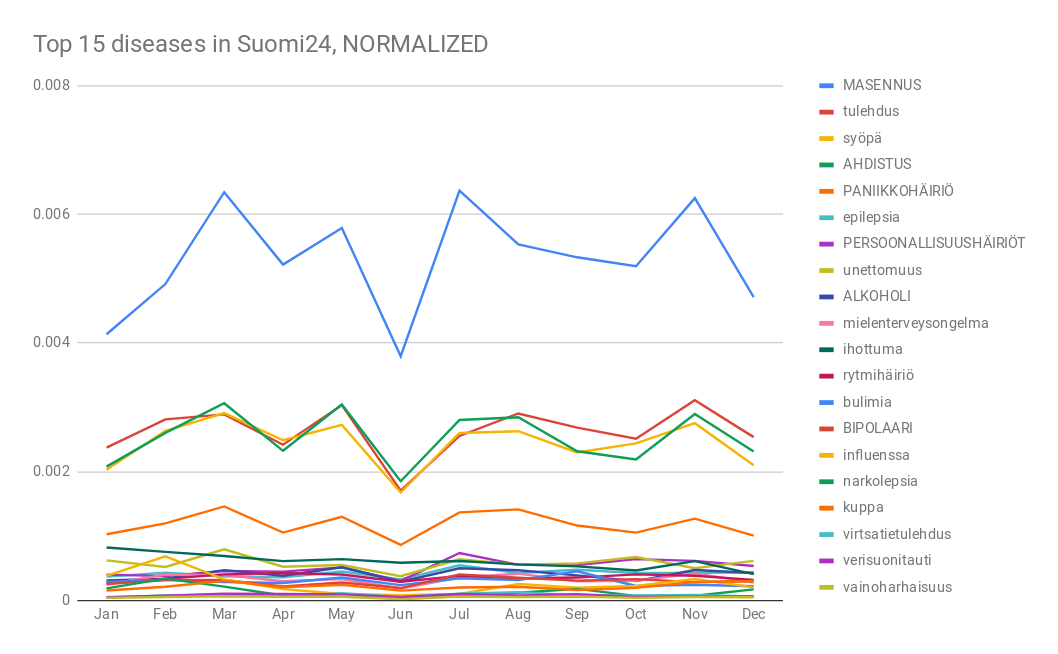
\includegraphics[width=0.45\textwidth]{figures/fig19.png}}
    \caption{Top 15 diseases in Suomi24, NORMALIZED}
    \label{top_15_diseases_in_suomi24_NORMALIZED}
\end{figure}

\begin{figure}[htbp]
    \centerline{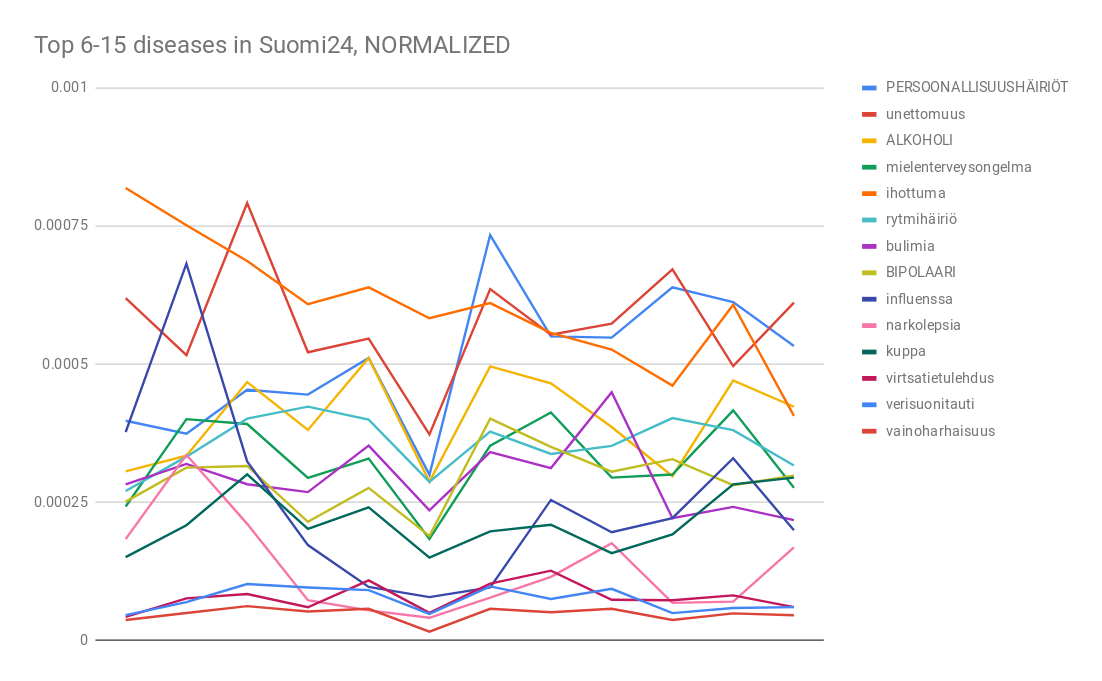
\includegraphics[width=0.45\textwidth]{figures/fig20.png}}
    \caption{Top 6-15 diseases in Suomi24, NORMALIZED}
    \label{top_6_15_diseases_in_suomi24_NORMALIZED}
\end{figure}

\section{Discussions}

\section{Conclusion}


\section*{Acknowledgment}

The preferred spelling of the word ``acknowledgment'' in America is without
an ``e'' after the ``g''. Avoid the stilted expression ``one of us (R. B.
G.) thanks $\ldots$''. Instead, try ``R. B. G. thanks$\ldots$''. Put sponsor
acknowledgments in the unnumbered footnote on the first page.

\bibliographystyle{IEEEtran}
\bibliography{IEEEabrv,mybibliography}

\end{document}
